
\documentclass{article}
\usepackage[landscape]{geometry}
\usepackage{url}
\usepackage{multicol}
\usepackage{array}
\usepackage{amsmath}
\usepackage{esint}
\usepackage{amsfonts}
\usepackage{tikz}
\usetikzlibrary{decorations.pathmorphing}
\usepackage{amsmath,amssymb}
\usepackage{bm}

\usepackage{colortbl}
\usepackage{xcolor}
\usepackage{mathtools}
\usepackage{amsmath,amssymb}
\usepackage{enumitem}
\usepackage{graphicx}
\makeatletter

\newcommand*\bigcdot{\mathpalette\bigcdot@{.5}}
\newcommand*\bigcdot@[2]{\mathbin{\vcenter{\hbox{\scalebox{#2}{$\m@th#1\bullet$}}}}}
\makeatother

\title{IND E 315 Cheat Sheet}
\usepackage[brazilian]{babel}
\usepackage[utf8]{inputenc}

\graphicspath{{./images/}}

\advance\topmargin-.8in
\advance\textheight3in
\advance\textwidth3in
\advance\oddsidemargin-1.5in
\advance\evensidemargin-1.5in
\parindent0pt
\parskip2pt
\newcommand{\hr}{\centerline{\rule{3.5in}{1pt}}}
%\colorbox[HTML]{e4e4e4}{\makebox[\textwidth-2\fboxsep][l]{texto}
\begin{document}

\begin{multicols*}{3}

\tikzstyle{mybox} = [draw=black, fill=white, very thick,
    rectangle, rounded corners, inner sep=10pt, inner ysep=10pt]
\tikzstyle{fancytitle} =[fill=black, text=white, font=\bfseries]

%------------ Events Content ---------------
\begin{tikzpicture}
    \node [mybox] (box){%
        \begin{minipage}{0.3\textwidth}
            \small{
                \begin{tabular}{lp{4.5cm} l}
                    \textbf{Union} & $E_1 \cup E_2$ \\ 
                                            & Events in \emph{either} event \\ 
                    \hline
                    \textbf{Intersection} & $E_1 \cap E_2$ \\
                                            & Events in \emph{both} events \\
                    \hline
                    \textbf{Complement} & $(E_1 \cup E_2)'$ \\
                                            & All events NOT in \emph{either} event \\
                    \hline
                    \textbf{Mutually exclusive} & $A \cap B = 0$ \\ 
                                            & Events share no common outcomes \\
                    \hline
                    \textbf{Independent} & $P(A|B) = P(A)$ \\ 
                                            & $P(B|A) = P(B)$ \\
                                            & $P(A \cap B) = P(A)P(B)$ \\
                                            & The occurrence of one event has no impact on the other
                \end{tabular}
            }
        \end{minipage}
    };
%------------ Events Header ---------------------
\node[fancytitle, right=10pt] at (box.north west) {Events - Terminology};
\end{tikzpicture}

%------------ Counting Techniques Content ---------------
\begin{tikzpicture}
    \node [mybox] (box){%
        \begin{minipage}{0.3\textwidth}
            \small{
                \begin{tabular}{lp{4.5cm} l}
                    \textbf{Multiplication Rule} & $n_1 * n_2 * \dots * n_k$ \\ 
                                            & Product gives total number of ways of completing steps 1 through k \\ 
                    \hline
                    \textbf{Permutation Rule} & $_nP_r = \frac{n!}{n_1! n_2! \dots n_r!}$ \\
                                            & Give number of permutations from ordered selection of $r$ objects from $n$ objects   \\
                                            & Sampling w/ replacement / Order matters   \\
                    \hline
                    \textbf{Combination Rule} & $_nC_r = \left( \begin{tabular}{c}
                        n \\
                        r
                        \end{tabular}  \right) = \frac{n!}{r!(n-r)!}$ \\ 
                                            & Give number of combinations from selection of (size) $r$ items from $n$ objects \\
                                            & Sampling w/o replacement / Order d/n matter \\
                \end{tabular}
            }
        \end{minipage}
    };
%------------ Counting Techniques Header ---------------------
\node[fancytitle, right=10pt] at (box.north west) {Counting Techniques};
\end{tikzpicture}

%------------ Random Variables Content ---------------
\begin{tikzpicture}
    \node [mybox] (box){%
        \begin{minipage}{0.3\textwidth}
            \small{
                \begin{tabular}{lp{3.5cm} l}
                    \textbf{Random Variables (rv)} & Function ($X$) that can take on values ($x$) for each outcome in a sample space \\
                    \hline
                    \textbf{Discrete rv's} & A random variable with a \emph{countable} range. \\
                                            & (counts, integers, or natural numbers) \\ 
                    \hline
                    \textbf{Continuous rv's} & A random variable with a \emph{uncountable} range. \\
                                            & (Such as length, weight, volume)
                \end{tabular}
            }
        \end{minipage}
    };
%------------ Random Variables Header ---------------------
\node[fancytitle, right=10pt] at (box.north west) {Random Variables};
\end{tikzpicture}


%------------ Probability Content ---------------
\begin{tikzpicture}
    \node [mybox] (box){%
        \begin{minipage}{0.3\textwidth}
            \small{
                \begin{tabular}{lp{4.8cm} l}
                    \textbf{Addition Rule} & \footnotesize{$P(A \cup B) = P(A) + P(B) - P(A \cap B)$} \\ 
                                            & \footnotesize{$P(A \cap B) = P(A) + P(B) - P(A \cup B)$} \\
                                            & If $P(A \cap B) =  0$, then \\
                                            & $P(A \cup B) = P(A) + P(B)$ \\
                    \hline
                    \textbf{Conditional Prob} & $P(B|A) = P(A \cap B) / P(A)$ \\
                                            & For $P(A) > 0$ \\ 
                                            & The conditional probability of event $B$ given event $A$ \\ 
                    \hline
                    \textbf{Multpl. Rule} & $P(A \cap B) = P(B|A) * P(A)$ \\
                                            & $P(B \cap A) = P(A|B) * P(B)$ \\
                                            & Probability of intersection \\
                    \hline
                    \textbf{Total Probability} & $P(B) = P(B \cap A) + P(B \cap A')$ \\ 
                                        & $P(B) = P(B|A) * P(A) + P(B|A') * P(A')$ \\
                                        & Sum of all events equals 1 \\
                    \hline
                    \textbf{Complement} & $P(A^C) = 1- P(A)$ \\ 
                                        & DeMorgan's Law: \\
                                        & $(A \cap B)' = A' \cup B' $ \\
                                        & $(A \cup B)' = A' \cap B' $ \\ 
                                        & Gives complements of a union or intersection \\
                \end{tabular}
            }
        \end{minipage}
    };
%------------ Probability Header ---------------------
\node[fancytitle, right=10pt] at (box.north west) {Probability};
\end{tikzpicture}

%\newpage

%------------ General Notes ---------------
\begin{tikzpicture}
    \node [mybox] (box){%
        \begin{minipage}{0.3\textwidth}
            Binomial - Given $n$ trials, count \# successes $x$ \\
            Geometric - Given 1 success, count \# trials $x$ \\
            Neg. Binomial - Given $r$ successes, count \# trials $x$ \\
            $P(A|B) \rightarrow $ (is) the probability of A occuring given B 
        \end{minipage}
    };
%------------ General Notes Header ---------------------
    \node[fancytitle, right=10pt] at (box.north west) {General Notes};
\end{tikzpicture}
    

%------------ Discrete Prob. Distribution Content ---------------
\begin{tikzpicture}
    \node [mybox] (box){%
        \begin{minipage}{0.64\textwidth}
            \small{
                %\fbox{
                    \begin{tabular}{  m{2.5cm} | m{4.5cm}| m{3.5cm} | m{5cm}} 
                        $\bm{X}$ & $\bm{f(x)}$ & $\bm{\mu = E(X)}$ & $\bm{\sigma ^2 = V(X)}$ \\ 
                        \hline
                        General          & $f(x_i) = P(X = x_i)$             & $\mu = \sum_x x * f(x)$              & $\sigma ^2 = V(X) = E(X - \mu)^2$\\
                        Uniform          & $f(x) = 1/(b - a + 1)$                  & $\mu = E(X) = (b + a)/2 $     & $\sigma ^2 = V(x) = ((b - a + 1)^2 - 1)/12 $\\     
                        Binomial         & $f(x) = _nC_x p^x (1 - p)^{n-x}$        & $\mu = E(X) = np$             & $\sigma ^2 = V(X) = np(1-p)$\\
                        Poisson          & $f(x) = (e^{-\lambda} \lambda ^x)/x!$        & $\mu = E(X) = \lambda$             & $\sigma ^2 = V(X) = \lambda$\\
                        Geometric        & $f(x) = p^1 (1-p)^{x-1}$                & $\mu = E(X) = 1/p$            & $\sigma ^2 = V(X) = (1-p)/(p^2)$\\
                        Neg. Binomial    & $f(x) = _{x-1}C_{r-1} p^r (1-p)^{x-r}$   & $\mu = E(X) = r/p$            & $\sigma ^2 = V(X) = (r(1-p))/(p^2)$\\
                        Hypr. Geometr    & $f(x) =$ \large{ $\frac{_{M}C_{x} * _{(N-M)}C_{(N-x)}}{_{N}C_{n}}$}     & $\mu = E(X) = M/N $           & $\sigma ^2 = V(X) = $\large{ $\frac{nM(N-M)(N-n)}{N^2(N-1)}$}\\
                    \end{tabular}
                %}
     
            }
        \end{minipage}
    };
%------------ Discrete Prob. Distribution Header ---------------------
\node[fancytitle, right=10pt] at (box.north west) {Discrete Prob. Distribution (General)};
\end{tikzpicture}

%------------ Continuous Prob. Distribution Content ---------------
\begin{tikzpicture}
    \node [mybox] (box){%
        \begin{minipage}{0.64\textwidth}
            \small{
                %\fbox{
                    \begin{tabular}{  m{2.5cm} | m{4.5cm}| m{3.5cm} | m{5cm}} 
                        $\bm{X}$ & $\bm{f(x)}$ & $\bm{\mu = E(X)}$ & $\bm{\sigma ^2 = V(X)}$ \\ 
                        \hline
                        %General          & $f(x_i) = P(X = x_i)$             & $\mu = \sum_x x * f(x)$              & $\sigma ^2 = V(X) = E(X - \mu)^2$\\
                        Uniform          & $f(x) = 1/(b - a)$                  & $\mu = E(X) = (b + a)/2 $     & $\sigma ^2 = V(x) = ((b - a)^2)/12 $\\     
                        Exponential      & $f(x) = (\lambda e^{-\lambda x})$        & $\mu = E(X) = 1/\lambda$             & $\sigma ^2 = V(X) = 1/(\lambda^2)$\\
                        Normal        & $f(x) =$ \large{ $\frac{1}{\sigma \sqrt{2 \pi}}e^{-0.5((x-\mu)/\sigma)^2}$} & $\mu = E(X) = \mu $ & $\sigma ^2 = V(X) = \sigma $\\
                        Standard Normal (Z)    & $f(x) =$ \large{ $\frac{1}{\sqrt{2 \pi}}e^{-0.5x^2}$}   & $\mu = E(X) = 0$ & $\sigma ^2 = V(X) = 1$\\
                        %Hypr. Geometr    & $f(x) =$ \large{ $\frac{_{M}C_{x} * _{(N-M)}C_{(N-x)}}{_{N}C_{n}}$}     & $\mu = E(X) = M/N $           & $\sigma ^2 = V(X) = $\large{ $\frac{nM(N-M)(N-n)}{N^2(N-1)}$}\\
                    \end{tabular}
                %}
     
            }
        \end{minipage}
    };
%------------ Continuous Prob. Distribution Header ---------------------
\node[fancytitle, right=10pt] at (box.north west) {Continuous Prob. Distribution (General)};
\end{tikzpicture}

%------------ Probability Content ---------------
\begin{tikzpicture}
    \node [mybox] (box){%
        \begin{minipage}{0.3\textwidth}
            \small{
                \begin{tabular}{lp{4.8cm} l}
                    \textbf{Probability Mass} & Describes the probability distribution of $X$. \\
                    \textit{(PMF, Discrete)}              \\
                    \hline

                    \textbf{Probability Dens.} & Describes the probability distribution of $X$. \\
                    \textit{(PDF, Continuous)} & Integrating w.r.t x gives you an area function for prob./dx * dx \\
                    \hline

                    \textit{Cumulative Dist.} & Describes the probability that $X$ will be less than or equal to $x$ \\
                    \textit{(CDF)}              & $F(x) = P(X \leq x)$ \\    
                    \textbf{(General)}          & $F(x) = \int^x_{lower} f(u) du$\\
                    \hline

                    \textit{Mean}               & Center of a probability distribution. \\
                    \hline

                    \textit{Variance}           & Varability in a probability distribution.\\ 
                    \textbf{(General)}          & $\sigma ^2 = \sum_x x^2 * f(x) - \mu ^2$, or \\
                                                & $\sigma ^2 = E[X^2] - (E[X])^2$, or \\
                                                & $\sigma ^2 = V(X) = E(X - \mu)^2$ \\ 


                \end{tabular}
            }
        \end{minipage}
    };
%------------ Probability Header ---------------------
\node[fancytitle, right=10pt] at (box.north west) {Probability Dist. Functions};
\end{tikzpicture}

%------------ Misc Properties Content ---------------
\begin{tikzpicture}
    \node [mybox] (box){%
        \begin{minipage}{0.3\textwidth}
            \small{
                \begin{tabular}{l l}
                    $E(aX) = aE(X)$          & (Continious) $P(X=x) = 0$   \\
                    $E(aX + b) = aE(X) + b$  & (Normal Dist.) $z = (x - \mu)/\sigma$   \\
                    $E[f(X)] = \sum f(x) p(x)$     \\
                    $V(aX) = a^2 V(X)$          \\
                    $V(aX + B) = a^2 V(X)$      \\
                \end{tabular}
            }
        \end{minipage}
    };
%------------ Misc Properties Header ---------------------
\node[fancytitle, right=10pt] at (box.north west) {Probability - Misc Properties};
\end{tikzpicture}

\newpage

\textbf{IND E 315 Cheat Sheet - Anthony Le}

%------------ Bayes Theorem Notes ---------------
\begin{tikzpicture}
    \node [mybox] (box){%
        \begin{minipage}{0.3\textwidth}
            $P(\text{Hypothesis Given Evidence}) \rightarrow P(H|E)$\\
            $P(H)$ ("Prior") represents probability of hypothesis being true before considering any new evidence \\
            $P(E|H)$ ("Likihood") represents probability of seeing evidence given hypothesis is true\\
            IE librarians fitting description \\
            $P(E|\neg H)$ represents probability of seeing evidence given hypothesis is false \\
            Bayes Theorem:\\
            $P(H|E) = \frac{(P(H))(P(E|H))}{(P(H))(P(E|H))+(P(\neg H))(P(E|\neg H))}$ \\
            Or alternatively:\\
             $P(H|E) = \frac{(P(H))(P(E|H))}{P(E)}$\\
            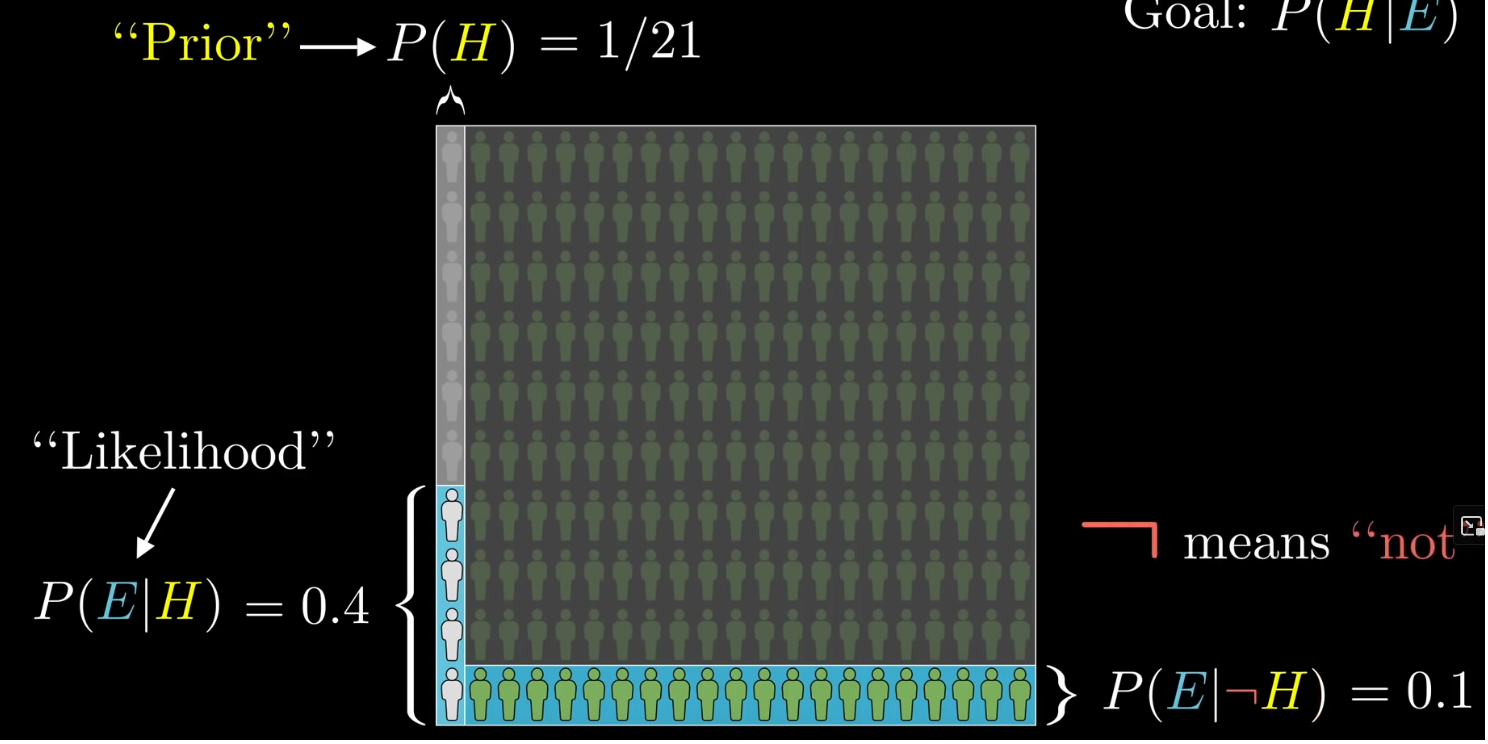
\includegraphics[width=7cm]{3B1B_BayesThrm}
        \end{minipage}
    };
%------------ General Notes Header ---------------------
    \node[fancytitle, right=10pt] at (box.north west) {General Notes};
\end{tikzpicture}



\end{multicols*}

\end{document}
